\documentclass{report}
\usepackage{graphicx}
\usepackage{fullpage}
\def\d{{\fontencoding{T1}\selectfont\dj}}
\def\D{{\fontencoding{T1}\selectfont\DJ}}

\author{
  Ro\v sko, Bojan\\
  \texttt{2013/0102 SI}
  \and
  Veinovi\' c, Relja\\
  \texttt{2013/0432 SI}
  }
\title{Doma\' ci zadatak 2015/2016:\\ Neuralne mre\v ze}
\date{26. januar 2016.\\[5\baselineskip] Sa\v zetak:\\[2\baselineskip]
Cilj ve\v zbe je obu\v cavanje perceptronske i vi\v seslojne feedforward neuralne mre\v ze za klasifikovanje podataka, kao i demonstracija tehnike ranog zaustavljanja.\\[2\baselineskip]
Zadatak je ra\d en sa podacima iz grupe 0, PodaciA1.txt i PodaciB1.txt, sa brojevima neurona po skrivenim slojevima ([8], [20], [3,8], [25,25]), i sa aktivacionim funkcijama po slojevima ('logsig','logsig')}
\begin{document}
\huge\maketitle\normalsize
\begin{enumerate}\LARGE

\item
Podaci A1:\large



\begin{center}
\begin{figure}[!h]
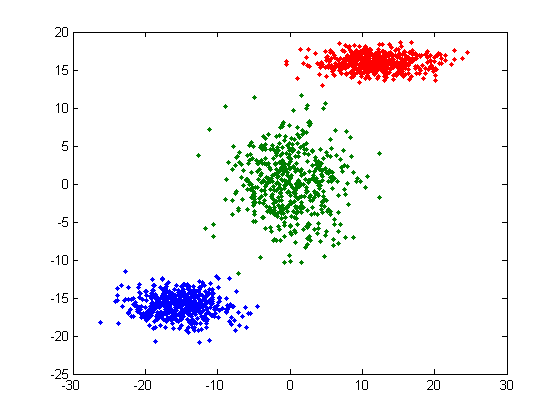
\includegraphics{A1input.png}
\caption{Podaci A1}
\end{figure}
\end{center}







\newpage
\begin{enumerate}
\item\LARGE
Perceptron:\large

\begin{figure}[!h]
\begin{center}
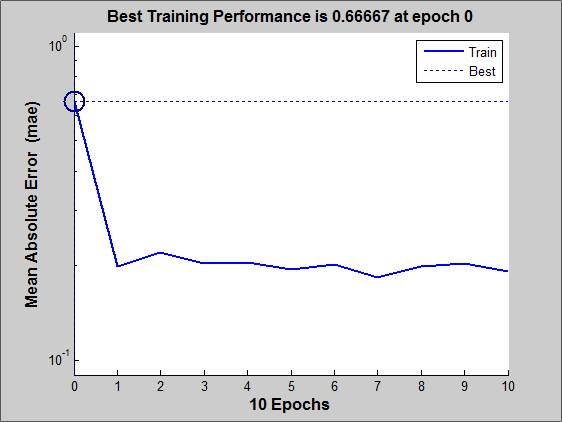
\includegraphics[scale=0.8]{A1performancePerceptron.png}
\caption{Performanse treniranja perceptrona}
\end{center}
\end{figure}

\begin{figure}[!h]
\begin{center}
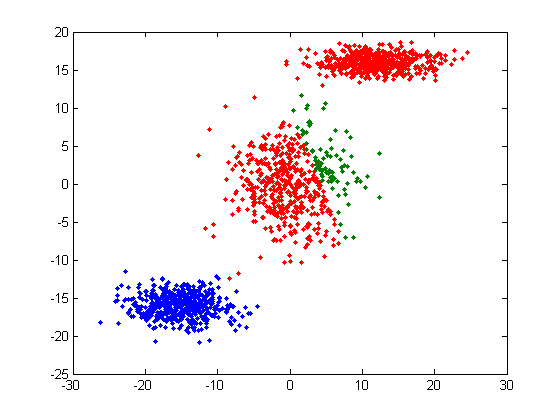
\includegraphics[scale=0.8]{A1outputPerceptronSame.png}
\caption{Izlaz perceptrona za iste ulazne podatke}
\end{center}
\end{figure}

\begin{figure}[!h]
\begin{center}
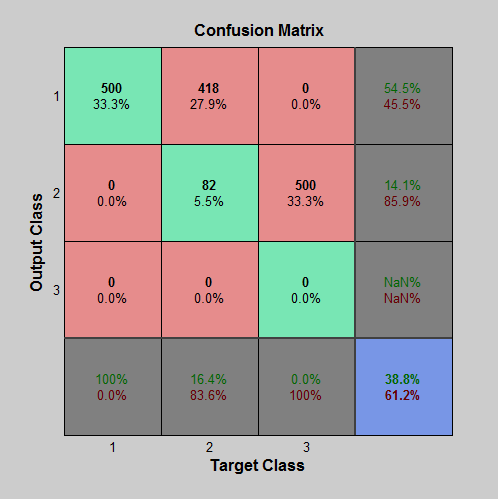
\includegraphics[scale=0.7]{A1confussionPerceptron.png}
\end{center}
\caption{Confussion matrix}
\end{figure}

\begin{figure}[!h]
\begin{center}
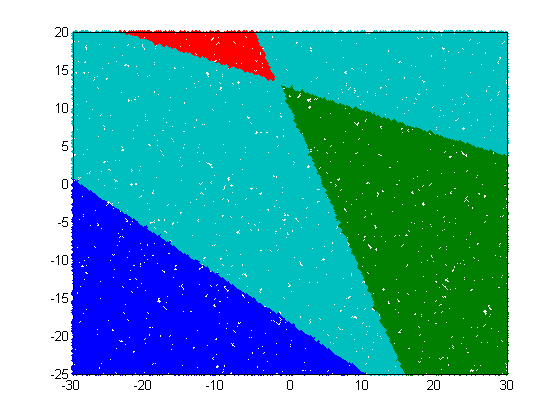
\includegraphics[scale=0.8]{A1outputPerceptronRandom50000.png}
\end{center}
\caption{Izlaz perceptrona na celom opsegu}
\end{figure}










\newpage
\item\LARGE
Feedforward 1 sa ranim zaustavljanjem:\large

\begin{figure}[!h]
\begin{center}
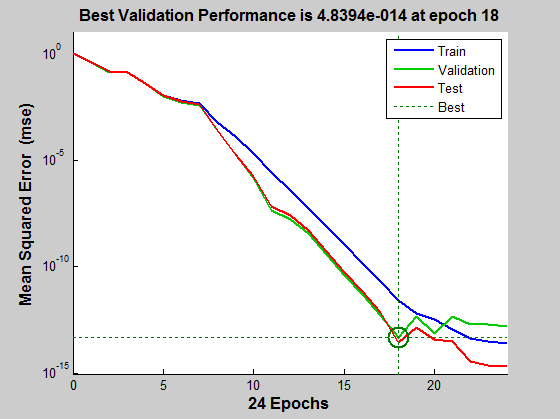
\includegraphics[scale=0.8]{A1performanceFF1early.png}
\caption{Performanse treniranja ff mreze sa ranim zaustavljanjem}
\end{center}
\end{figure}

\begin{figure}[!h]
\begin{center}
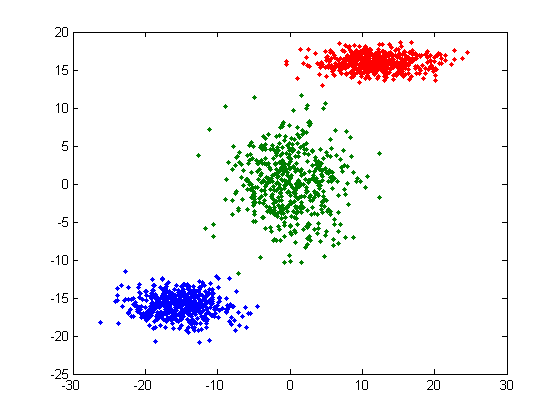
\includegraphics[scale=0.8]{A1outputFF1earlySame.png}
\caption{Izlaz ff mreze za iste ulazne podatke}
\end{center}
\end{figure}

\begin{figure}[!h]
\begin{center}
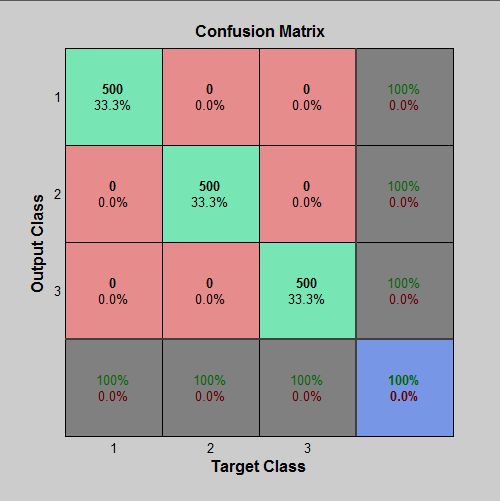
\includegraphics[scale=0.7]{A1confussionFF1early.png}
\caption{Confusion matrix}
\end{center}
\end{figure}

\begin{figure}[!h]
\begin{center}
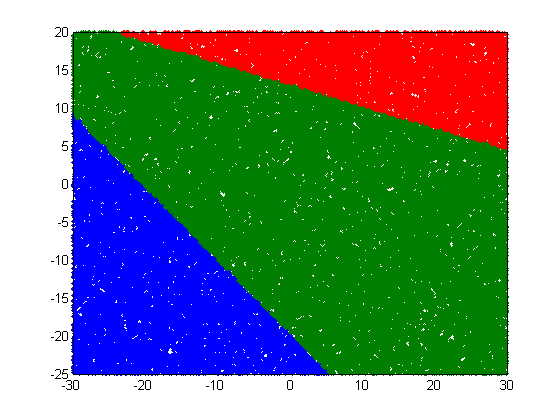
\includegraphics[scale=0.8]{A1outputFF1earlyRandom50000.png}
\caption{Izlaz ff mreze na celom opsegu}
\end{center}
\end{figure}

\newpage
\item\LARGE
Feedforward 1 bez ranog zaustavljanja:\large

\begin{figure}[!h]
\begin{center}
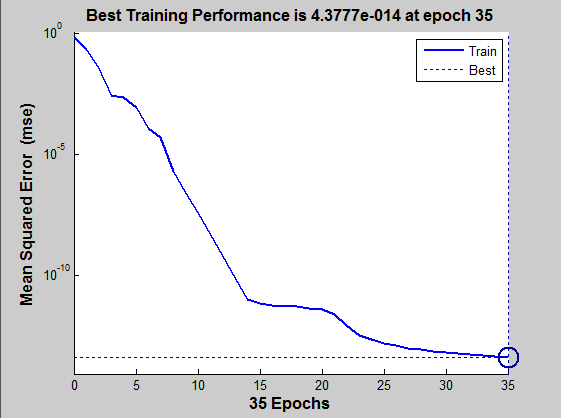
\includegraphics[scale=0.8]{A1performanceFF1.png}
\caption{Performanse treniranja ff mreze sa ranim zaustavljanjem}
\end{center}
\end{figure}

\begin{figure}[!h]
\begin{center}
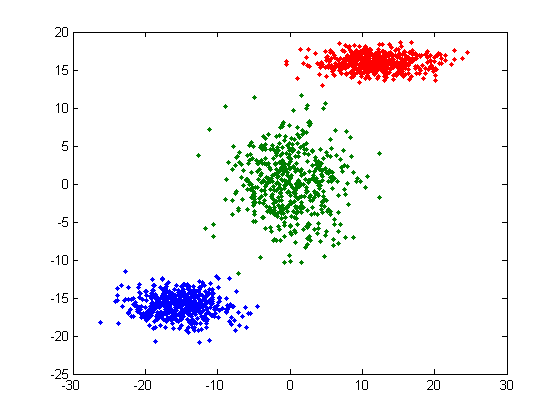
\includegraphics[scale=0.8]{A1outputFF1earlySame.png}
\caption{Izlaz ff mreze za iste ulazne podatke}
\end{center}
\end{figure}

\begin{figure}[!h]
\begin{center}
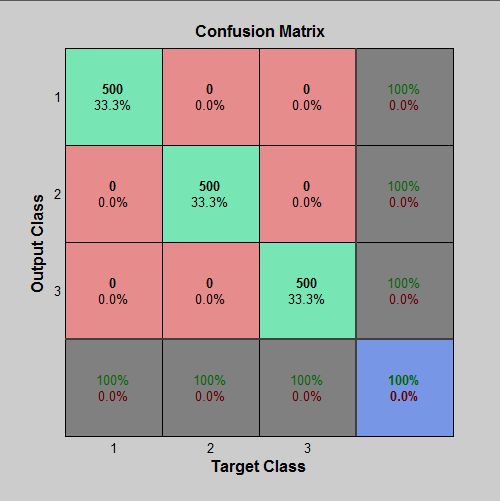
\includegraphics[scale=0.7]{A1confussionFF1early.png}
\caption{Confusion matrix}
\end{center}
\end{figure}

\begin{figure}[!h]
\begin{center}
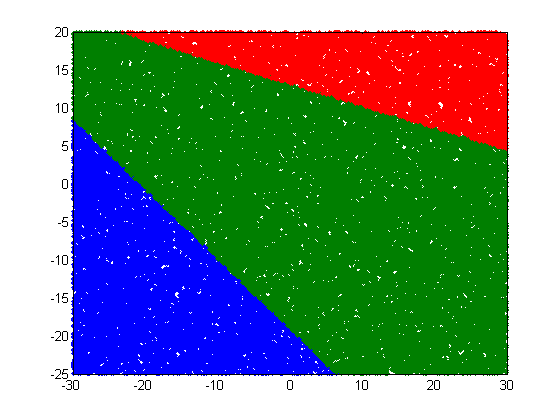
\includegraphics[scale=0.8]{A1outputFF1Random50000.png}
\caption{Izlaz ff mreze na celom opsegu}
\end{center}
\end{figure}









\newpage
\item\LARGE
Feedforward 2 sa ranim zaustavljanjem:\large

\begin{figure}[!h]
\begin{center}
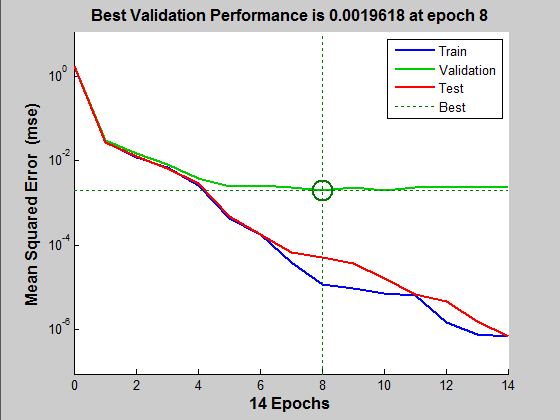
\includegraphics[scale=0.8]{A1performanceFF2early.png}
\caption{Performanse treniranja ff mreze sa ranim zaustavljanjem}
\end{center}
\end{figure}

\begin{figure}[!h]
\begin{center}
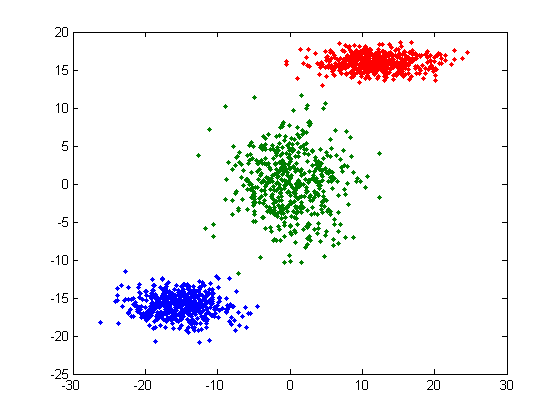
\includegraphics[scale=0.8]{A1outputFF1earlySame.png}
\caption{Izlaz ff mreze za iste ulazne podatke}
\end{center}
\end{figure}

\begin{figure}[!h]
\begin{center}
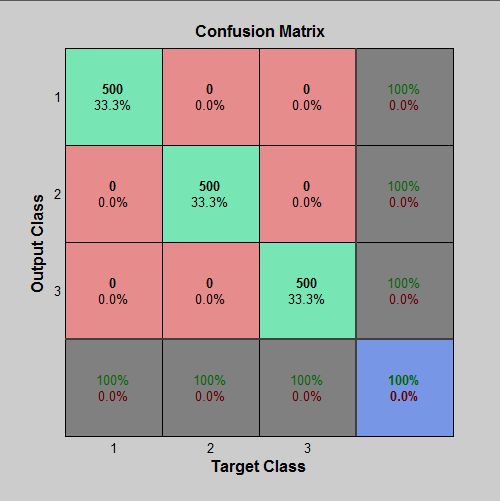
\includegraphics[scale=0.7]{A1confussionFF1early.png}
\caption{Confusion matrix}
\end{center}
\end{figure}

\begin{figure}[!h]
\begin{center}
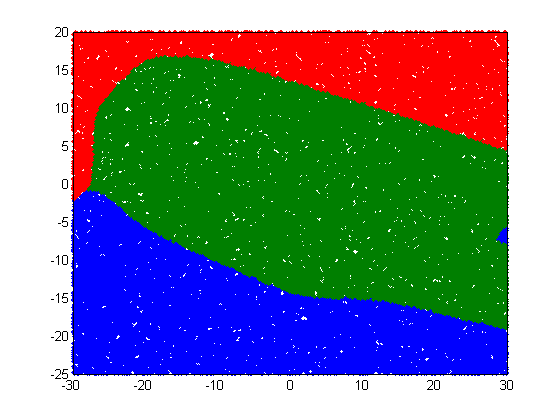
\includegraphics[scale=0.8]{A1outputFF2earlyRandom50000.png}
\caption{Izlaz ff mreze na celom opsegu}
\end{center}
\end{figure}

\newpage
\item\LARGE
Feedforward 2 bez ranog zaustavljanja:\large

\begin{figure}[!h]
\begin{center}
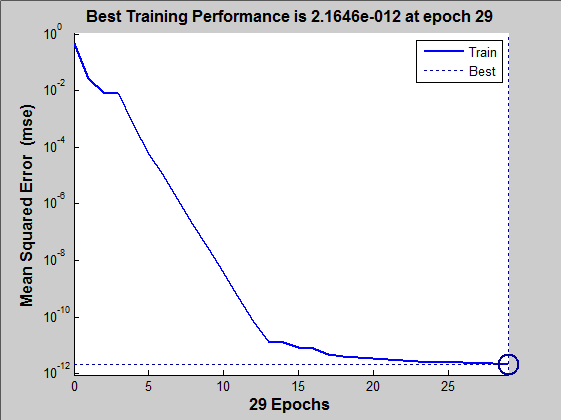
\includegraphics[scale=0.8]{A1performanceFF2.png}
\caption{Performanse treniranja ff mreze sa ranim zaustavljanjem}
\end{center}
\end{figure}

\begin{figure}[!h]
\begin{center}
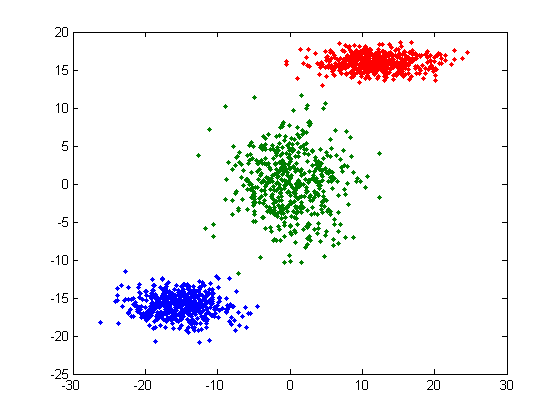
\includegraphics[scale=0.8]{A1outputFF1earlySame.png}
\caption{Izlaz ff mreze za iste ulazne podatke}
\end{center}
\end{figure}

\begin{figure}[!h]
\begin{center}
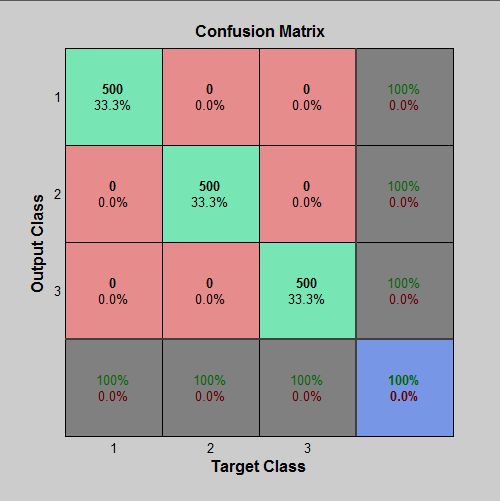
\includegraphics[scale=0.7]{A1confussionFF1early.png}
\caption{Confusion matrix}
\end{center}
\end{figure}

\begin{figure}[!h]
\begin{center}
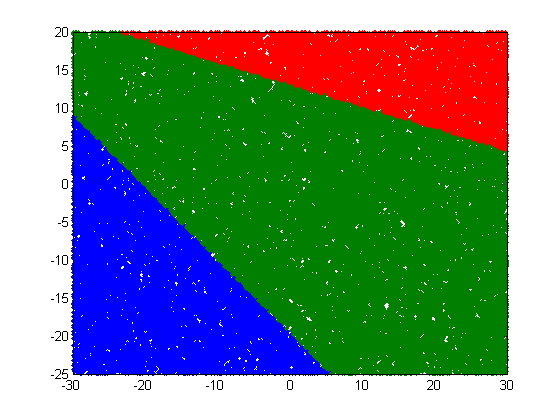
\includegraphics[scale=0.8]{A1outputFF2Random50000.png}
\caption{Izlaz ff mreze na celom opsegu}
\end{center}
\end{figure}









\newpage
\item\LARGE
Feedforward 3 sa ranim zaustavljanjem:\large

\begin{figure}[!h]
\begin{center}
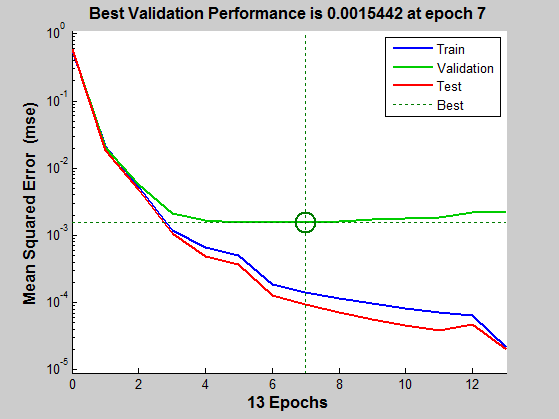
\includegraphics[scale=0.8]{A1performanceFF3early.png}
\caption{Performanse treniranja ff mreze sa ranim zaustavljanjem}
\end{center}
\end{figure}

\begin{figure}[!h]
\begin{center}
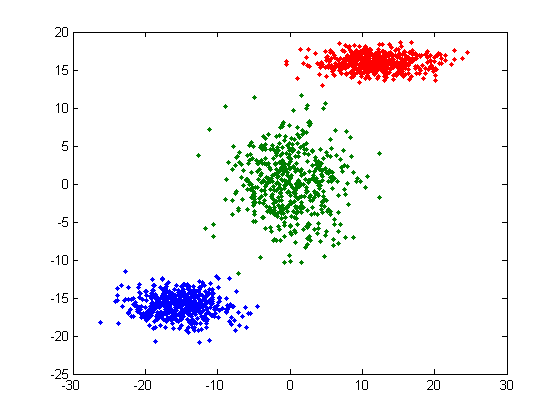
\includegraphics[scale=0.8]{A1outputFF1earlySame.png}
\caption{Izlaz ff mreze za iste ulazne podatke}
\end{center}
\end{figure}

\begin{figure}[!h]
\begin{center}
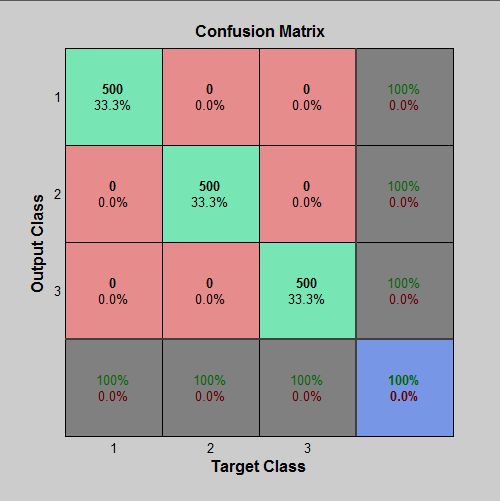
\includegraphics[scale=0.7]{A1confussionFF1early.png}
\caption{Confusion matrix}
\end{center}
\end{figure}

\begin{figure}[!h]
\begin{center}
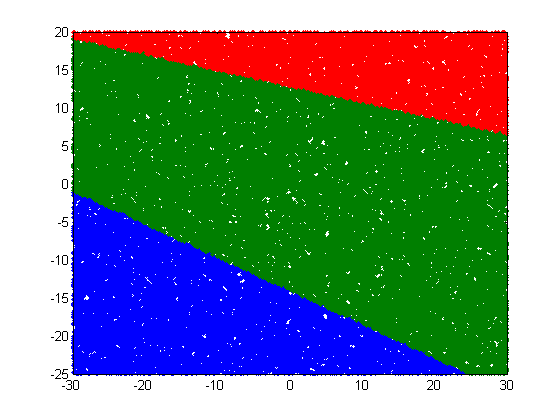
\includegraphics[scale=0.8]{A1outputFF3earlyRandom50000.png}
\caption{Izlaz ff mreze na celom opsegu}
\end{center}
\end{figure}

\newpage
\item\LARGE
Feedforward 3 bez ranog zaustavljanja:\large

\begin{figure}[!h]
\begin{center}
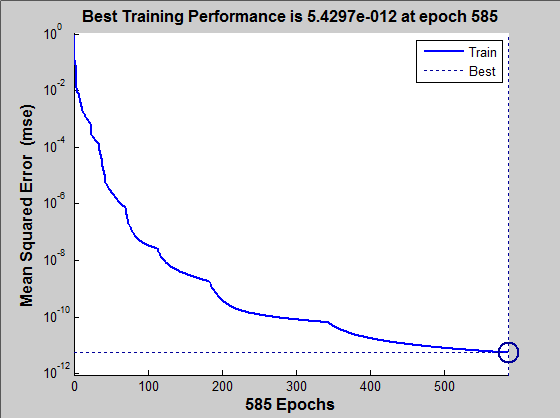
\includegraphics[scale=0.8]{A1performanceFF3.png}
\caption{Performanse treniranja ff mreze sa ranim zaustavljanjem}
\end{center}
\end{figure}

\begin{figure}[!h]
\begin{center}
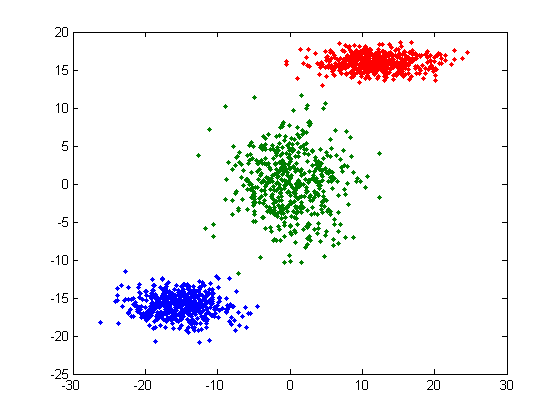
\includegraphics[scale=0.8]{A1outputFF1earlySame.png}
\caption{Izlaz ff mreze za iste ulazne podatke}
\end{center}
\end{figure}

\begin{figure}[!h]
\begin{center}
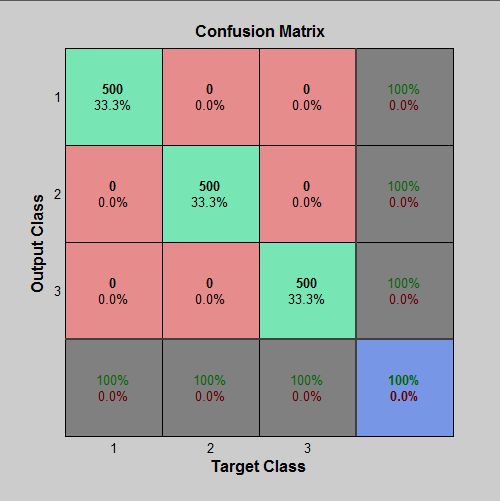
\includegraphics[scale=0.7]{A1confussionFF1early.png}
\caption{Confusion matrix}
\end{center}
\end{figure}

\begin{figure}[!h]
\begin{center}
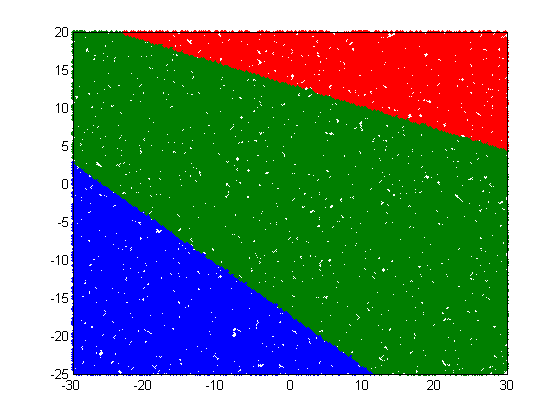
\includegraphics[scale=0.8]{A1outputFF3Random50000.png}
\caption{Izlaz ff mreze na celom opsegu}
\end{center}
\end{figure}










\newpage
\item\LARGE
Feedforward 4 sa ranim zaustavljanjem:\large

\begin{figure}[!h]
\begin{center}
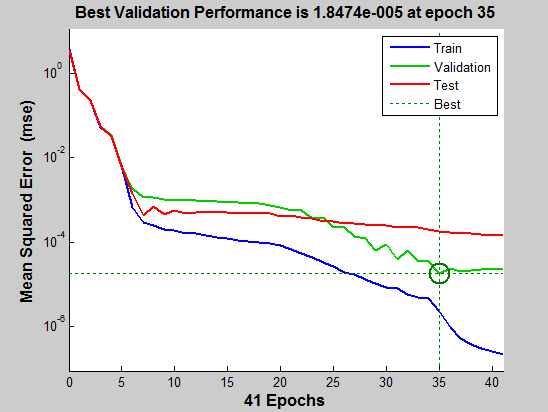
\includegraphics[scale=0.8]{A1performanceFF4early.png}
\caption{Performanse treniranja ff mreze sa ranim zaustavljanjem}
\end{center}
\end{figure}

\begin{figure}[!h]
\begin{center}
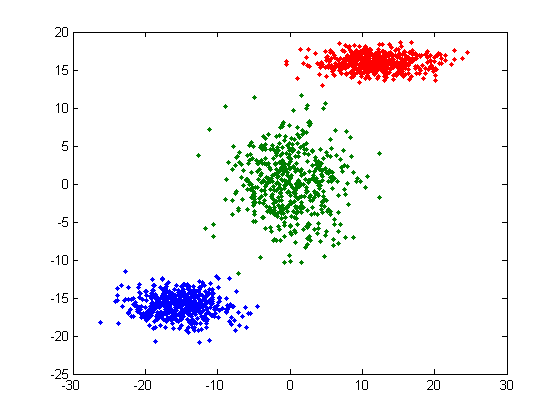
\includegraphics[scale=0.8]{A1outputFF1earlySame.png}
\caption{Izlaz ff mreze za iste ulazne podatke}
\end{center}
\end{figure}

\begin{figure}[!h]
\begin{center}
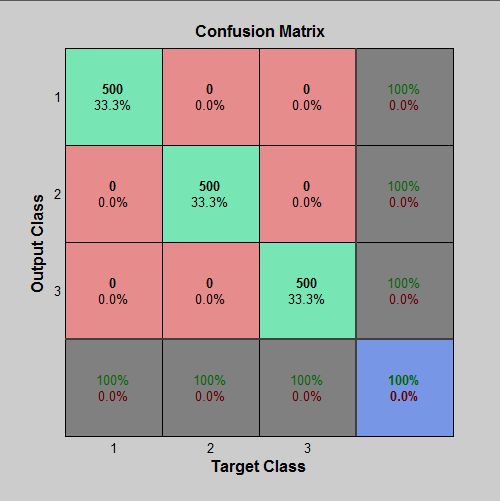
\includegraphics[scale=0.7]{A1confussionFF1early.png}
\caption{Confusion matrix}
\end{center}
\end{figure}

\begin{figure}[!h]
\begin{center}
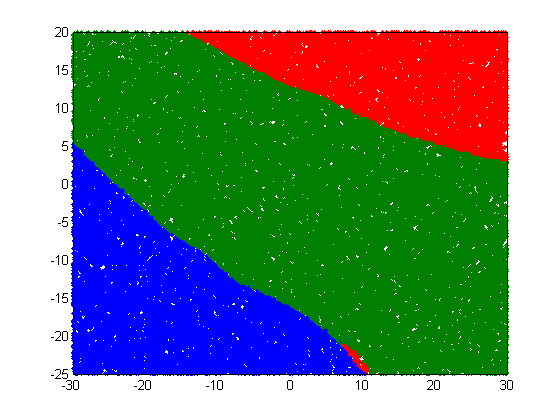
\includegraphics[scale=0.8]{A1outputFF4earlyRandom50000.png}
\caption{Izlaz ff mreze na celom opsegu}
\end{center}
\end{figure}

\newpage
\item\LARGE
Feedforward 4 bez ranog zaustavljanja:\large

\begin{figure}[!h]
\begin{center}
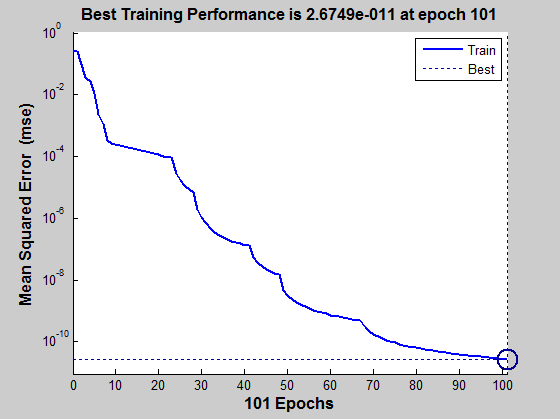
\includegraphics[scale=0.8]{A1performanceFF4.png}
\caption{Performanse treniranja ff mreze sa ranim zaustavljanjem}
\end{center}
\end{figure}

\begin{figure}[!h]
\begin{center}
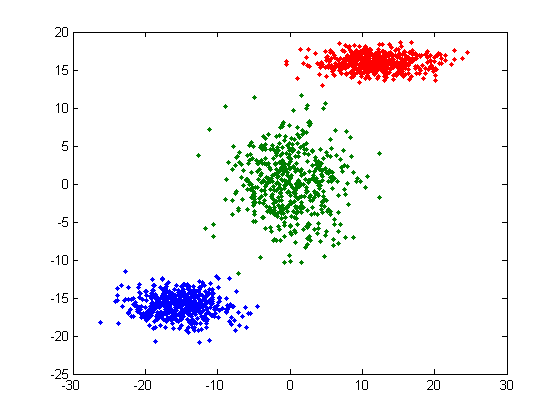
\includegraphics[scale=0.8]{A1outputFF1earlySame.png}
\caption{Izlaz ff mreze za iste ulazne podatke}
\end{center}
\end{figure}

\begin{figure}[!h]
\begin{center}
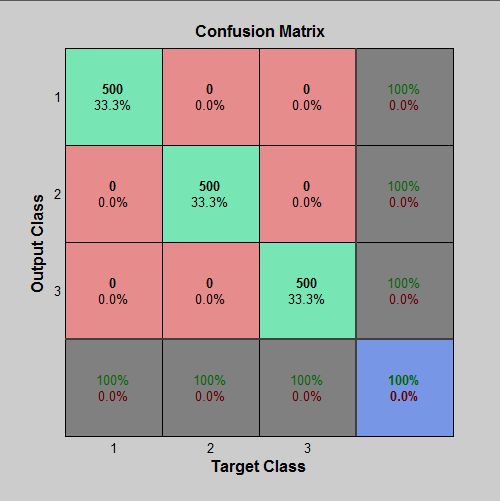
\includegraphics[scale=0.7]{A1confussionFF1early.png}
\caption{Confusion matrix}
\end{center}
\end{figure}

\begin{figure}[!h]
\begin{center}
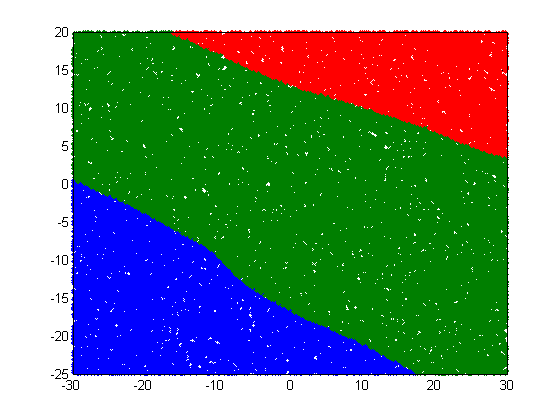
\includegraphics[scale=0.8]{A1outputFF4Random50000.png}
\caption{Izlaz ff mreze na celom opsegu}
\end{center}
\end{figure}



\end{enumerate}




\newpage
\LARGE
\item
Podaci B1:\large





\begin{center}
\begin{figure}[!h]
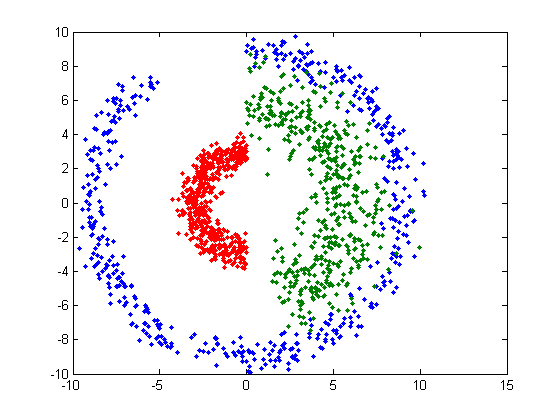
\includegraphics{B1input.png}
\caption{Podaci B1}
\end{figure}
\end{center}







\newpage
\begin{enumerate}
\item\LARGE
Perceptron:\large

\begin{figure}[!h]
\begin{center}
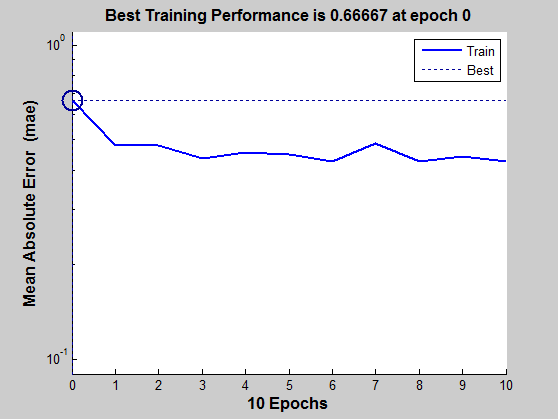
\includegraphics[scale=0.8]{B1performancePerceptron.png}
\caption{Performanse treniranja perceptrona}
\end{center}
\end{figure}

\begin{figure}[!h]
\begin{center}
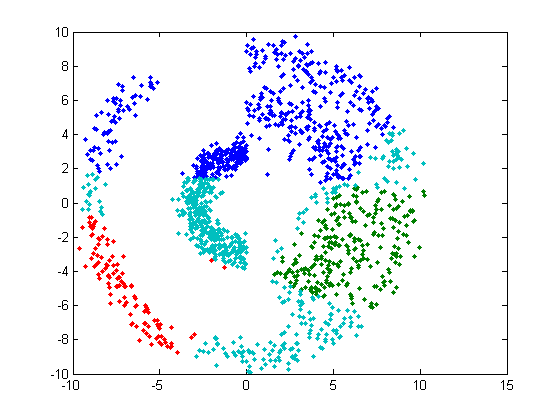
\includegraphics[scale=0.8]{B1outputPerceptronSame.png}
\caption{Izlaz perceptrona za iste ulazne podatke}
\end{center}
\end{figure}

\begin{figure}[!h]
\begin{center}
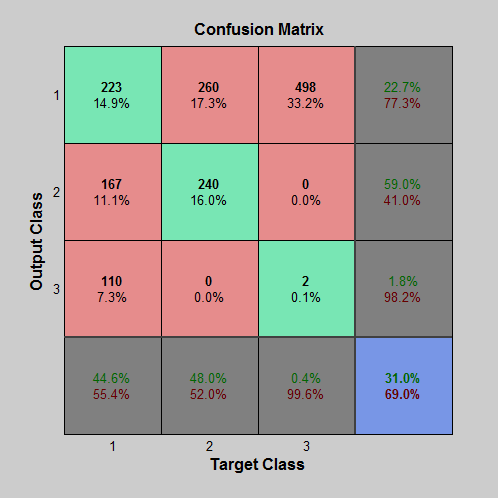
\includegraphics[scale=0.7]{B1confussionPerceptron.png}
\end{center}
\caption{Confussion matrix}
\end{figure}

\begin{figure}[!h]
\begin{center}
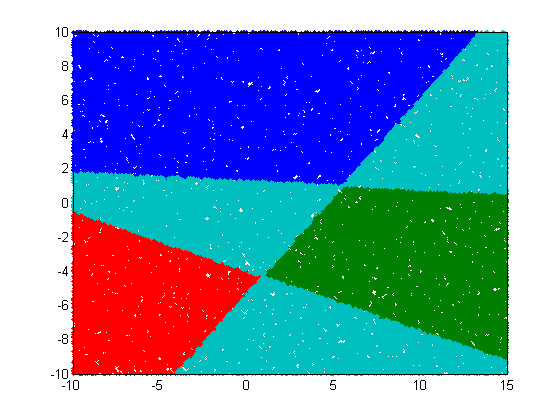
\includegraphics[scale=0.8]{B1outputPerceptronRandom50000.png}
\end{center}
\caption{Izlaz perceptrona na celom opsegu}
\end{figure}










\newpage
\item\LARGE
Feedforward 1 sa ranim zaustavljanjem:\large

\begin{figure}[!h]
\begin{center}
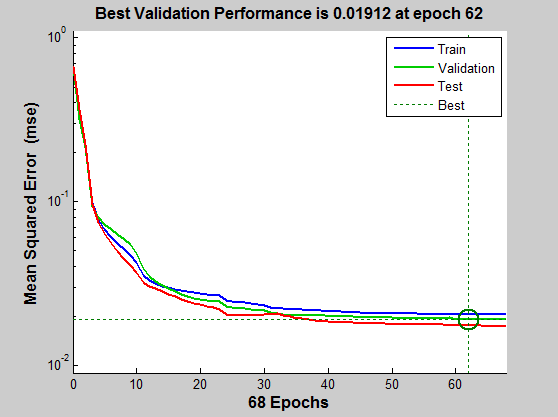
\includegraphics[scale=0.8]{B1performanceFF1early.png}
\caption{Performanse treniranja ff mreze sa ranim zaustavljanjem}
\end{center}
\end{figure}

\begin{figure}[!h]
\begin{center}
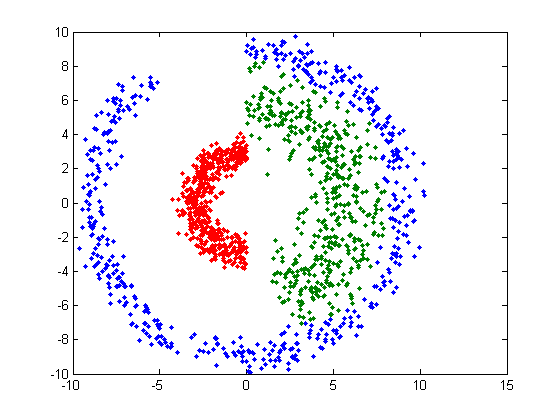
\includegraphics[scale=0.8]{B1outputFF1earlySame.png}
\caption{Izlaz ff mreze za iste ulazne podatke}
\end{center}
\end{figure}

\begin{figure}[!h]
\begin{center}
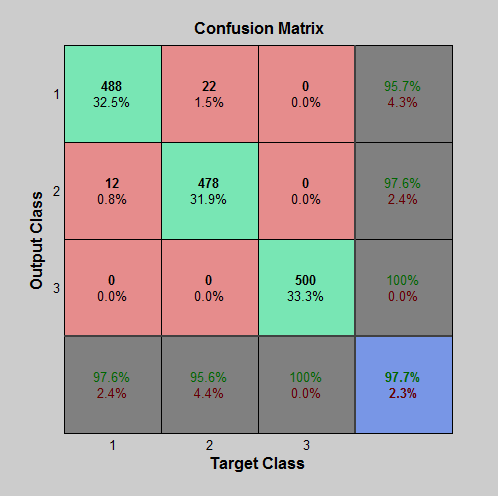
\includegraphics[scale=0.7]{B1confussionFF1early.png}
\caption{Confusion matrix}
\end{center}
\end{figure}

\begin{figure}[!h]
\begin{center}
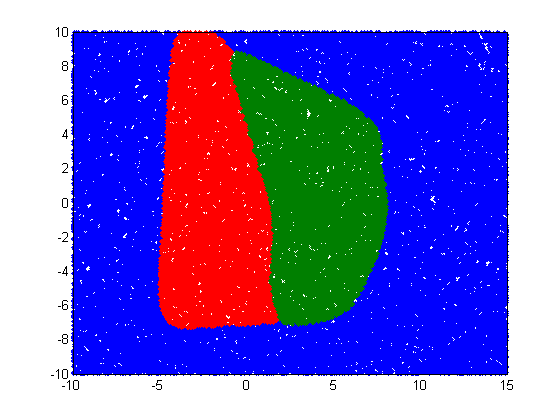
\includegraphics[scale=0.8]{B1outputFF1earlyRandom50000.png}
\caption{Izlaz ff mreze na celom opsegu}
\end{center}
\end{figure}

\newpage
\item\LARGE
Feedforward 1 bez ranog zaustavljanja:\large

\begin{figure}[!h]
\begin{center}
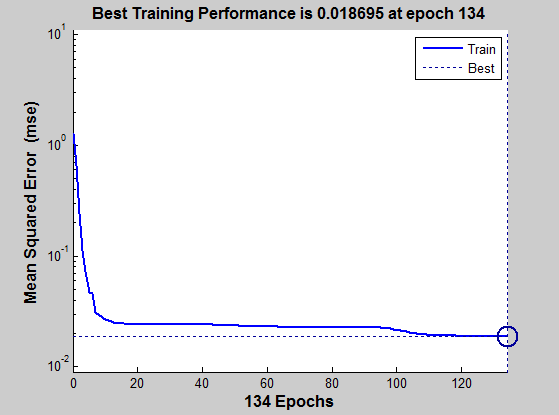
\includegraphics[scale=0.8]{B1performanceFF1.png}
\caption{Performanse treniranja ff mreze sa ranim zaustavljanjem}
\end{center}
\end{figure}

\begin{figure}[!h]
\begin{center}
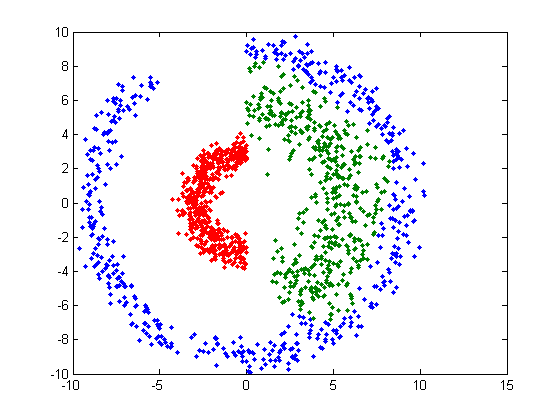
\includegraphics[scale=0.8]{B1outputFF1Same.png}
\caption{Izlaz ff mreze za iste ulazne podatke}
\end{center}
\end{figure}

\begin{figure}[!h]
\begin{center}
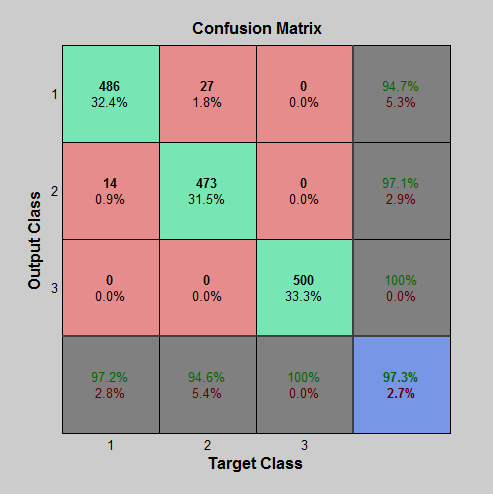
\includegraphics[scale=0.7]{B1confussionFF1.png}
\caption{Confusion matrix}
\end{center}
\end{figure}

\begin{figure}[!h]
\begin{center}
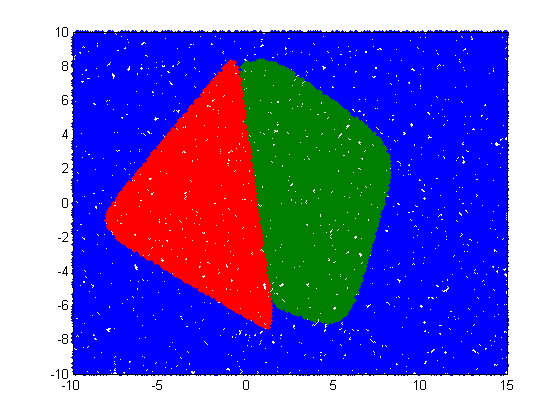
\includegraphics[scale=0.8]{B1outputFF1Random50000.png}
\caption{Izlaz ff mreze na celom opsegu}
\end{center}
\end{figure}









\newpage
\item\LARGE
Feedforward 2 sa ranim zaustavljanjem:\large

\begin{figure}[!h]
\begin{center}
\includegraphics[scale=0.8]{B1performanceFF2early.png}
\caption{Performanse treniranja ff mreze sa ranim zaustavljanjem}
\end{center}
\end{figure}

\begin{figure}[!h]
\begin{center}
\includegraphics[scale=0.8]{B1outputFF2earlySame.png}
\caption{Izlaz ff mreze za iste ulazne podatke}
\end{center}
\end{figure}

\begin{figure}[!h]
\begin{center}
\includegraphics[scale=0.7]{B1confussionFF2early.png}
\caption{Confusion matrix}
\end{center}
\end{figure}

\begin{figure}[!h]
\begin{center}
\includegraphics[scale=0.8]{B1outputFF2earlyRandom50000.png}
\caption{Izlaz ff mreze na celom opsegu}
\end{center}
\end{figure}

\newpage
\item\LARGE
Feedforward 2 bez ranog zaustavljanja:\large

\begin{figure}[!h]
\begin{center}
\includegraphics[scale=0.8]{B1performanceFF2.png}
\caption{Performanse treniranja ff mreze sa ranim zaustavljanjem}
\end{center}
\end{figure}

\begin{figure}[!h]
\begin{center}
\includegraphics[scale=0.8]{B1outputFF2Same.png}
\caption{Izlaz ff mreze za iste ulazne podatke}
\end{center}
\end{figure}

\begin{figure}[!h]
\begin{center}
\includegraphics[scale=0.7]{B1confussionFF2.png}
\caption{Confusion matrix}
\end{center}
\end{figure}

\begin{figure}[!h]
\begin{center}
\includegraphics[scale=0.8]{B1outputFF2Random50000.png}
\caption{Izlaz ff mreze na celom opsegu}
\end{center}
\end{figure}









\newpage
\item\LARGE
Feedforward 3 sa ranim zaustavljanjem:\large

\begin{figure}[!h]
\begin{center}
\includegraphics[scale=0.8]{B1performanceFF3early.png}
\caption{Performanse treniranja ff mreze sa ranim zaustavljanjem}
\end{center}
\end{figure}

\begin{figure}[!h]
\begin{center}
\includegraphics[scale=0.8]{B1outputFF3earlySame.png}
\caption{Izlaz ff mreze za iste ulazne podatke}
\end{center}
\end{figure}

\begin{figure}[!h]
\begin{center}
\includegraphics[scale=0.7]{B1confussionFF3early.png}
\caption{Confusion matrix}
\end{center}
\end{figure}

\begin{figure}[!h]
\begin{center}
\includegraphics[scale=0.8]{B1outputFF3earlyRandom50000.png}
\caption{Izlaz ff mreze na celom opsegu}
\end{center}
\end{figure}

\newpage
\item\LARGE
Feedforward 3 bez ranog zaustavljanja:\large

\begin{figure}[!h]
\begin{center}
\includegraphics[scale=0.8]{B1performanceFF3.png}
\caption{Performanse treniranja ff mreze sa ranim zaustavljanjem}
\end{center}
\end{figure}

\begin{figure}[!h]
\begin{center}
\includegraphics[scale=0.8]{B1outputFF3Same.png}
\caption{Izlaz ff mreze za iste ulazne podatke}
\end{center}
\end{figure}

\begin{figure}[!h]
\begin{center}
\includegraphics[scale=0.7]{B1confussionFF3.png}
\caption{Confusion matrix}
\end{center}
\end{figure}

\begin{figure}[!h]
\begin{center}
\includegraphics[scale=0.8]{B1outputFF3Random50000.png}
\caption{Izlaz ff mreze na celom opsegu}
\end{center}
\end{figure}










\newpage
\item\LARGE
Feedforward 4 sa ranim zaustavljanjem:\large

\begin{figure}[!h]
\begin{center}
\includegraphics[scale=0.8]{B1performanceFF4early.png}
\caption{Performanse treniranja ff mreze sa ranim zaustavljanjem}
\end{center}
\end{figure}

\begin{figure}[!h]
\begin{center}
\includegraphics[scale=0.8]{B1outputFF4earlySame.png}
\caption{Izlaz ff mreze za iste ulazne podatke}
\end{center}
\end{figure}

\begin{figure}[!h]
\begin{center}
\includegraphics[scale=0.7]{B1confussionFF4early.png}
\caption{Confusion matrix}
\end{center}
\end{figure}

\begin{figure}[!h]
\begin{center}
\includegraphics[scale=0.8]{B1outputFF4earlyRandom50000.png}
\caption{Izlaz ff mreze na celom opsegu}
\end{center}
\end{figure}

\newpage
\item\LARGE
Feedforward 4 bez ranog zaustavljanja:\large

\begin{figure}[!h]
\begin{center}
\includegraphics[scale=0.8]{B1performanceFF4.png}
\caption{Performanse treniranja ff mreze sa ranim zaustavljanjem}
\end{center}
\end{figure}

\begin{figure}[!h]
\begin{center}
\includegraphics[scale=0.8]{B1outputFF4Same.png}
\caption{Izlaz ff mreze za iste ulazne podatke}
\end{center}
\end{figure}

\begin{figure}[!h]
\begin{center}
\includegraphics[scale=0.7]{B1confussionFF4.png}
\caption{Confusion matrix}
\end{center}
\end{figure}

\begin{figure}[!h]
\begin{center}
\includegraphics[scale=0.8]{B1outputFF4Random50000.png}
\caption{Izlaz ff mreze na celom opsegu}
\end{center}
\end{figure}



\end{enumerate}



\end{enumerate}

\end{document}